\documentclass{elektr}
\usepackage[OT1]{fontenc}
\usepackage{hyperref}
\hypersetup{
    colorlinks=true,
    urlcolor=black,
    citecolor=blue,
    linkcolor=black
}
\usepackage{amsfonts,amssymb,amsmath,amsgen,amsopn,amsbsy,theorem,graphicx}
\usepackage{eufrak,amscd,bezier,latexsym,enumerate}
\usepackage[utf8]{inputenc}
\usepackage[english]{babel}
\usepackage{multirow}
\usepackage[dvipsnames]{xcolor}
\usepackage{tikz}
\usetikzlibrary{shapes.geometric,arrows,positioning,fit,calc}

\yil{2026}
\vol{34}
\fpage{1}
\lpage{15}
\doi{10.3906/elk-2606-1}

\title{An explainable end-to-end log anomaly detection framework for distributed

systems}

\author[BEKKOUCHE et al.]{
	\textbf{Mohammed BEKKOUCHE$^{1,}$\thanks{m.bekkouche@esi-sba.dz}, Adem TOUMI$^{1}$, Sidi Mohammed BENSLIMANE$^{1}$}\\
	$^{1}$LabRI-SBA Lab., Ecole Superieure en Informatique, Sidi Bel Abbes, Algeria\\\\
	Mohammed BEKKOUCHE: \url{https://orcid.org/0000-0002-1245-7895} \\
	Adem TOUMI: \url{https://orcid.org/0000-0002-8145-2367} \\
	Sidi Mohammed BENSLIMANE: \url{https://orcid.org/0000-0001-9876-5432}\\ [1.8em]
	\rec{12.06.2026}
	\acc{28.06.2026}
	\finv{}
}

\input{elksty.tex}

\makeatletter
\DeclareFontFamily{T1}{cmr}{}
\DeclareFontShape{T1}{cmr}{m}{n}{<-> cmr10}{}
\DeclareFontShape{T1}{cmr}{bx}{n}{<-> cmbx10}{}
\DeclareFontShape{T1}{cmr}{m}{it}{<-> cmti10}{}
\DeclareFontFamily{TS1}{cmr}{}
\DeclareFontShape{TS1}{cmr}{m}{n}{<-> cmr10}{}
\DeclareFontShape{TS1}{cmr}{bx}{n}{<-> cmbx10}{}
\makeatother

\begin{document}

\maketitle

\begin{abstract}
Log-based anomaly detection in distributed systems is hindered by three systemic
limitations: single-benchmark evaluation that obscures generalizability, inadequate
handling of extreme class imbalance, and opaque model predictions that impede
operational diagnosis. We present a comprehensive comparative study that simultaneously
addresses all three limitations.

We implement ten model architectures across four paradigms---supervised classifiers,
supervised sequential deep learning, unsupervised reconstruction, and transformer
language models---and evaluate selected architecture--dataset combinations on the
HDFS, BGL, and Spirit benchmarks under a rigorous five-invariant zero-leakage
experimental protocol. A critical distinction governs the evaluation: supervised
models (SVM, Decision Tree, Random Forest, CNN+BiLSTM, Attention-BiLSTM,
DeepLog Enhanced, LogBERT, LogGPT2) are trained with full anomaly labels, while
the proposed unsupervised Bidirectional LSTM Autoencoder (BiLSTM-AE) is trained
exclusively on normal-class sessions---requiring \emph{no anomaly labels whatsoever}.
To address the scarcity of labeled anomalies, we design the BiLSTM-AE with trainable
dense log-key embeddings and validation-driven $F_1$-sensitive threshold optimization.
Operating without any labeled anomalies, the proposed BiLSTM-AE achieves
$F_1{=}0.9571$ with perfect recall ($\text{Recall}{=}1.0000$) on HDFS, surpassing
DeepLog by $+0.2280$ under identical chronological evaluation. Supervised classifiers
achieve near-perfect detection ($F_1{=}0.9962$ on BGL, $F_1{=}0.9999$ on Spirit)
at sub-millisecond latency. The BiLSTM-AE is further equipped with post-hoc
explainability via SHAP and LIME, yielding domain-consistent feature attributions
aligned with expert knowledge of BGL failure tokens. A deployed REST API and
Streamlit dashboard complete the operational cycle.
\keywords{log anomaly detection; distributed systems; explainable AI; LSTM
autoencoder; temporally consistent evaluation; cross-dataset generalization; SHAP; LIME}
\end{abstract}

\section{Introduction}
\label{Sec:Intro}

Distributed computing systems (cloud platforms, microservices, HPC clusters)
coordinate thousands of components. This complexity enables scalability but
multiplies the fault propagation surface: misconfigurations or hardware faults
can cascade rapidly. System logs are the primary observability source, recording
component states, severity levels, and execution traces. At large scales, logs
accumulate at rates exceeding gigabytes per hour~\cite{ref13}, rendering manual
inspection infeasible.

Automated log anomaly detection has evolved from rule-based matching to
machine and deep learning~\cite{ref4,ref5}. However, three systemic
challenges limit production adoption.

\textbf{Challenge 1---Cross-dataset generalization.} Most studies evaluate only
on a single benchmark, typically HDFS~\cite{ref5,ref7,ref18}. Performance on
datasets with different log structures or anomaly types (e.g., BGL hardware
events or Spirit supercomputer logs) remains largely untested, leaving
generalizability unverified.

\textbf{Challenge 2---Class imbalance.} Real-world anomaly rates are severely
skewed: 2.93\% for HDFS and 7.34\% for BGL at the session and line levels,
respectively; Spirit's window-level rate appears higher (32.04\%) due to the
windowed detection unit construction rather than a higher underlying fault density.
Training protocols that ignore this skew yield models with high accuracy but poor
recall, failing to surface actual faults to operators.

\textbf{Challenge 3---Model opacity.} Modern neural networks output anomaly
alerts without explanation. SREs must manually triage flagged logs, increasing
Mean Time to Resolution (MTTR). Explainable AI (XAI) methods that identify
anomaly-driving tokens are essential for practical deployment.

To address all three challenges, this paper makes the following four contributions:

\begin{itemize}
    \item \textbf{C1: Unified Zero-Leakage Protocol.}
    A five-invariant evaluation protocol preventing temporal data leakage enables
    reproducible cross-dataset comparison of ten model architectures across
    four paradigms on HDFS, BGL, and Spirit.

    \item \textbf{C2: Optimized Unsupervised BiLSTM-AE.}
    An unsupervised Bidirectional LSTM Autoencoder trained exclusively on normal
    sessions. It uses trainable dense log-key embeddings ($d{=}64$) and
    $F_1$-sensitive threshold optimization to achieve competitive HDFS performance without labeled anomalies.

    \item \textbf{C3: Representation--Anomaly Alignment Principle.}
    The first empirical demonstration, validated across all three standard benchmarks,
    that sequential dense-embedding representations dominate on session-order anomalies
    (HDFS) while sparse TF-IDF representations dominate on content-localized anomalies
    (BGL, Spirit)---providing an actionable model-selection guideline absent from prior work.

    \item \textbf{C4: Deployed Explainability Layer.}
    SHAP~\cite{ref9} and LIME~\cite{ref10} are integrated into a FastAPI backend
    and Streamlit dashboard. The BiLSTM-AE also features a native,
    zero-overhead explainability signal via per-timestep reconstruction error.
\end{itemize}

\textbf{Experimental setting.} Two complementary operating regimes are evaluated.
\emph{Supervised setting}: SVM, Decision Tree, Random Forest, CNN+BiLSTM,
Attention-BiLSTM, DeepLog Enhanced, LogBERT, and LogGPT2 are trained with full
binary anomaly labels; these represent the reference upper bound. \emph{Unsupervised setting}: the proposed BiLSTM-AE is
trained exclusively on normal-class sessions and detects anomalies purely via
reconstruction error. Comparisons should be read as complementary regimes, not a
performance competition: the question is whether the label-free BiLSTM-AE
provides viable detection when anomaly labels are unavailable.

The remainder of the paper is organized as follows. Section~\ref{Sec:Related}
reviews related work. Section~\ref{Sec:Preprocessing} describes datasets and
protocol. Section~\ref{Sec:Framework} presents model architectures.
Section~\ref{Sec:Results} reports results, revealing that representation choice
matters as much as model family on line-level benchmarks.
Section~\ref{Sec:XAI} covers the integrated explainability analysis.
Section~\ref{Sec:Deployment} describes the deployed system.
Section~\ref{Sec:Conclusion} concludes.

\section{Background and Related Work}
\label{Sec:Related}

Log anomaly detection typically involves three sequential steps: log parsing,
feature engineering, and classification or reconstruction.

\subsection{Log Parsing and Feature Representation}

Raw system logs are free-form text. The Drain parser~\cite{ref6} converts log
streams into structured templates online using a fixed-depth parse tree at high
throughput. Parsed logs are projected into vector spaces using one of four
representations: (i)~Event Count Matrices (ECM)~\cite{ref4}, accumulating
per-template frequencies within a detection window; (ii)~TF-IDF sparse
vectors~\cite{ref1}, weighting tokens by discriminativity across sessions;
(iii)~Log-key sequences~\cite{ref5}, preserving chronological template identifiers;
and (iv)~Word2Vec semantic embeddings~\cite{ref2}, projecting templates into a
dense semantic space by exploiting co-occurrence statistics.

\subsection{Anomaly Detection Methods}

\textbf{Supervised and Self-supervised Methods.}
He et al.~\cite{ref4} established ML baselines (SVM, Isolation Forest~\cite{ref12}) on
HDFS ECM representations. DeepLog~\cite{ref5} reformulates detection as next-log-key
prediction via LSTM, flagging sessions where the observed key falls outside the
top-$g$ predictions; it trains on normal data only and is therefore self-supervised.
LogRobust~\cite{ref17} addresses log instability with
attention mechanisms and FastText embeddings. LogBERT~\cite{ref18} adapts a
BERT-based transformer via masked log-key prediction. Bekkouche and Benslimane~\cite{ref1}
demonstrated that the train-test split strategy is the dominant factor explaining
HDFS performance variance---a finding that directly motivates our zero-leakage
protocol.

\textbf{Unsupervised Reconstruction.}
LogAnomaly~\cite{ref7} uses template2vec embeddings and a BiLSTM to model
both sequential and quantitative log patterns. Bekkouche et al.~\cite{ref2}
showed that a BiLSTM Autoencoder achieves $F_1{=}0.993$ on HDFS under a random
(non-chronological) split---a figure not directly comparable to zero-leakage evaluations. Wu et al.~\cite{ref8} conducted the most comprehensive representation
study to date across HDFS, BGL, and Spirit.

\textbf{LLM and Graph-based Approaches.}
Generative language models, such as LogLLM~\cite{ref23} and LogGPT~\cite{ref24} (evaluated in this work as LogGPT2), fine-tune pretrained transformers on log sequences to achieve strong cross-dataset detection, while graph-based frameworks like DeepTraLog~\cite{ref22} model distributed trace dependencies via Graph Neural Networks. Zhu et al.~\cite{ref25} propose CoLA, a collaborative framework that combines a lightweight detection model with an LLM to improve both detection accuracy and explainability. Sui et al.~\cite{ref26} address cross-system generalization through LogSynergy, which uses LLM-based log interpretation and unified feature extraction to transfer anomaly detection knowledge to new software systems with limited labeled data. Hadadi et al.~\cite{ref27} introduce FlexLog, which combines several machine learning classifiers with a retrieval-augmented LLM to maintain detection performance on unstable log data while reducing labeling requirements. In contrast, our work focuses on an unsupervised reconstruction-based approach that does not require labeled anomaly data, making it complementary to these LLM-based methods.

\subsection{Explainability Gap}

Despite the critical operational need for actionable anomaly explanations, no prior
work has systematically integrated post-hoc XAI frameworks into an end-to-end log
anomaly detection pipeline evaluated across multiple standard benchmarks. SHAP and
LIME have been applied to general NLP classification but remain absent from
multi-dataset log anomaly evaluation. Table~\ref{tab:gap_analysis} positions our
work against the closest related methods on five key dimensions.

\begin{table}[h!]
\caption{Systematic gap analysis positioning our work against the closest
related methods. DS\,=\,multi-dataset; Imb\,=\,imbalance-aware; ZL\,=\,zero-leakage;
XAI\,=\,explainability; Dep\,=\,deployment demonstration.}
\begin{center}
\small
\begin{tabular}{|p{2.3cm}|c|c|c|c|c|}
\hline
\textbf{Method} & \textbf{DS} & \textbf{Imb} & \textbf{ZL} & \textbf{XAI} & \textbf{Dep} \\
\hline
DeepLog \cite{ref5}      & No  & No  & No  & No  & No  \\
LogBERT \cite{ref18}     & No  & No  & No  & No  & No  \\
LogRobust \cite{ref17}   & No  & Yes & No  & No  & No  \\
Wu et al. \cite{ref8}    & Yes & No  & No  & No  & No  \\
Bekkouche \cite{ref2}    & No  & Yes & No  & No  & No  \\
\textbf{Ours}            & \textbf{Yes} & \textbf{Yes} & \textbf{Yes} & \textbf{Yes} & \textbf{Yes} \\
\hline
\end{tabular}
\label{tab:gap_analysis}
\end{center}\vs{-4mm}
\end{table}

\section{Preprocessing and Zero-Leakage Protocol}
\label{Sec:Preprocessing}

\subsection{Datasets}

We evaluate on three public benchmarks of complementary character.
\textbf{HDFS} (v1)~\cite{ref13}: Hadoop distributed file system logs from a 203-node Amazon
EC2 cluster, yielding a Drain-parsed CSV of 2.612\,GB.
Block identifiers define natural session boundaries; anomaly rate 2.93\%.
\textbf{BGL}~\cite{ref15}: BlueGene/L HPC system logs; the Drain-parsed CSV is
1.125\,GB. Hardware faults are annotated at the line level; anomaly rate 7.34\%.
\textbf{Spirit}~\cite{ref3,ref14}: Spirit supercomputer logs;
the Drain-parsed CSV is 1.067\,GB.
No session keys exist; window-level anomaly rate 32.04\%.

\subsection{Detection Unit Construction}

We design three dataset-specific grouping strategies.
\textbf{HDFS}: block-ID session grouping; a session is anomalous if any constituent
line is flagged.
\textbf{BGL}: single-line evaluation, as hardware alerts are self-contained.
\textbf{Spirit}: sliding window of size $W{=}20$ lines and stride $S{=}10$.
Table~\ref{tab:preprocessing} summarizes outcomes; Figure~\ref{fig:pipeline}
depicts the full pipeline.

\subsection{Zero-Leakage Protocol}

We define \emph{zero-leakage} as the property that all feature encoders and
decision thresholds are fitted exclusively on training data, with test-set labels
never accessed before final evaluation. Motivated by Le and Zhang~\cite{ref21} and
Bekkouche and Benslimane~\cite{ref1}, who showed that random splitting inflates
HDFS $F_1$ by up to 27 percentage points over chronological splitting, we enforce
five invariants:
(I1)~TF-IDF and Word2Vec encoders are fitted exclusively on training data;
(I2)~BGL and Spirit use a stratified random split (70/10/20\%); HDFS uses a
chronological split (60/20/20\%) for deep classifiers. For the BiLSTM-AE, a two-stage stratified splitting strategy was applied: first, 90\% of the data was reserved for training and validation, while 10\% was used for testing; the training-validation subset was then further divided into 90\% training and 10\% validation, resulting in an approximate 81/9/10 train-validation-test split (81\% training, 9\% validation, 10\% testing), as its normal-only training requires a larger
training fraction;
(I3)~session and window grouping is performed before partitioning to prevent
session-boundary leakage;
(I4)~class weights and anomaly thresholds are calibrated exclusively on
training/validation data;
(I5)~test labels are accessed only at final evaluation.
All random number generators (Python \texttt{random}, NumPy, PyTorch,
scikit-learn) are anchored to $\text{seed}=42$, ensuring exact reproducibility.
Single-run evaluation was governed by dataset scale ($>$4.75M log lines) and the
per-model Optuna budgets (Section~\ref{Sec:Limitations}).

\begin{table}[h!]
\caption{Preprocessing outcomes across the three benchmark datasets.}
\begin{center}
\small
\begin{tabular}{|p{2.0cm}|p{3.6cm}|p{3.6cm}|p{3.6cm}|}
\hline
\textbf{Property} & \textbf{HDFS} & \textbf{BGL} & \textbf{Spirit} \\
\hline
Detection unit &
Block session (variable length) &
Individual log line &
Sliding window ($W{=}20$, $S{=}10$) \\
\hline
Split strategy &
Temporal (60/20/20) / Stratified (81/9/10) &
Stratified 70/10/20 &
Stratified 70/10/20 \\
\hline
Feature repr. &
Word2Vec seq.\ + ECM &
TF-IDF (5{,}000 feats) &
TF-IDF (500 feats) + W2V \\
\hline
Anomaly rate &
2.93\% &
7.34\% &
32.04\%$^\dagger$ \\
\hline
Imbalance strategy &
Cost-sensitive loss &
Class weighting &
Class weighting \\
\hline
Output scale &
$\approx$575{,}000 sessions &
$\approx$4{,}750{,}000 lines &
$\approx$500{,}000 windows \\
\hline
\end{tabular}
\label{tab:preprocessing}
\smallskip\\
{\footnotesize $^\dagger$Window-level rate; higher than BGL/HDFS due to windowed
detection unit construction, not higher underlying fault density.}
\end{center}\vs{-4mm}
\end{table}

The design rationale follows from the structural characteristics of each dataset.
\textbf{Detection unit}: HDFS block sessions are naturally delimited by block
identifiers; BGL line-level annotations preclude aggregation without diluting
sparse hardware faults; Spirit sliding windows ($W{=}20$, $S{=}10$) provide
sequence context without natural session boundaries.
\textbf{Features}: trainable log-key embeddings + ECM for HDFS target
sequential execution-order anomalies; TF-IDF for BGL and Spirit targets
content-localized fault tokens---the empirical basis of Contribution C3.
\textbf{Imbalance}: cost-sensitive weighted cross-entropy for HDFS deep models;
\texttt{class\_weight=`balanced'} for BGL and Spirit classifiers.

\begin{figure}[h!]
\begin{center}
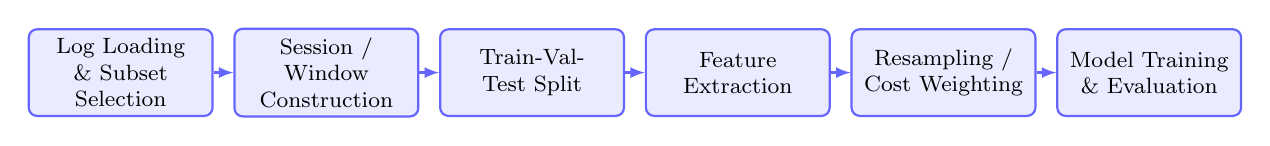
\begin{tikzpicture}[
    node distance=0.15cm and 0.25cm,
    block/.style={rectangle, draw=blue!60, fill=blue!8, thick,
                  text width=2.1cm, align=center, rounded corners=3pt,
                  minimum height=1.1cm, font=\footnotesize},
    line/.style={draw, -latex, thick, blue!60}
]
    \node [block] (load)  {Log Loading \& Subset Selection};
    \node [block, right=of load]  (group) {Session / Window Construction};
    \node [block, right=of group] (split) {Train-Val-Test Split};
    \node [block, right=of split] (feat)  {Feature Extraction};
    \node [block, right=of feat]  (imb)   {Resampling / Cost Weighting};
    \node [block, right=of imb]   (train) {Model Training \& Evaluation};
    
    \path [line] (load)  -- (group);
    \path [line] (group) -- (split);
    \path [line] (split) -- (feat);
    \path [line] (feat)  -- (imb);
    \path [line] (imb)   -- (train);
\end{tikzpicture}
\caption{The six-stage preprocessing and modeling pipeline enforcing the
zero-leakage protocol. Feature extractors (TF-IDF, Word2Vec) are fitted
exclusively on the training partition; the test partition remains isolated
until final evaluation.}
\label{fig:pipeline}
\end{center}\vs{-4mm}
\end{figure}

\section{Proposed Framework and Model Architectures}
\label{Sec:Framework}

\subsection{Problem Formulation}

Let $\mathcal{L}=\{l_1,\ldots,l_N\}$ be a raw log stream of $N$ log lines.
A parser $\mathcal{P}$ maps each line $l_i$ to a structured template
$e_i\in\mathcal{E}$, where $\mathcal{E}$ is the finite set of unique event
types (templates) discovered by the Drain parser. A grouping function
$\mathcal{G}$ partitions the stream into $K$ detection units
$u_k=(e_{k,1},\ldots,e_{k,|u_k|})$, where $|u_k|$ denotes the variable length
of unit $k$ (session length for HDFS, 1 for BGL, window size $W$ for Spirit).
A representation function $\phi: u_k\mapsto\mathbf{x}_k\in\mathbb{R}^d$ projects
each detection unit into a $d$-dimensional feature vector. A classifier
$f_\theta:\mathbb{R}^d\mapsto\mathbb{R}$ parameterized by weights $\theta$ outputs
a real-valued logit; the anomaly probability is $p_k = \sigma(f_\theta(\mathbf{x}_k))$,
where $\sigma(\cdot)$ is the sigmoid function, and the binary label is
$\hat{y}_k = \mathbf{1}[p_k > \delta]$ for a tuned threshold $\delta$.
A ground-truth label $y_k\in\{0,1\}$ is available for training supervised models.

To counteract class imbalance, supervised training minimizes the weighted
cross-entropy loss over all $K$ training units:
\begin{equation}
\mathcal{L}_{\text{cls}} = -\sum_{k=1}^{K}\bigl[
    w_1 y_k\log p_k + w_0(1{-}y_k)\log(1{-}p_k)\bigr],
\label{eq:cls_loss}
\end{equation}
where: $K$ is the number of training detection units; $y_k\in\{0,1\}$ is the
ground-truth label for unit $k$; $p_k$ is the predicted anomaly probability (as defined above);
$w_1 = \sqrt{N_0/N_1}$ is the anomaly-class weight proportional to the square root of the class-frequency ratio;
$w_0 = 1$ is the majority-class weight set to unity; $N_0$ is the count of normal units
and $N_1$ the count of anomalous units in the training partition.
Since anomalies are rare, $w_1 \gg w_0$, ensuring that gradient updates are dominated by the minority anomaly class rather than the abundant normal class.

For the unsupervised BiLSTM-AE, which trains exclusively on normal-class sessions
(no labels used), the model learns a normal-behavior manifold by minimizing mean
session reconstruction error. The input sequence for session $k$ is denoted
$\mathbf{E}^{(k)}=\bigl(\mathbf{e}^{(k)}_1,\ldots,\mathbf{e}^{(k)}_{L_k}\bigr)$,
where $\mathbf{e}^{(k)}_i\in\mathbb{R}^d$ is the trainable dense embedding
($d{=}64$) of the $i$-th log event in session $k$, and $L_k$ is the session
length. The reconstructed sequence is
$\hat{\mathbf{E}}^{(k)}=\bigl(\hat{\mathbf{e}}^{(k)}_1,\ldots,\hat{\mathbf{e}}^{(k)}_{L_k}\bigr)$.
The training objective is the mean squared reconstruction error (MSE) over all
$K_{\mathrm{tr}}$ normal training sessions:
\begin{equation}
\mathcal{L}_{\text{MSE}} = \frac{1}{K_{\mathrm{tr}}}\sum_{k=1}^{K_{\mathrm{tr}}}
\frac{1}{L_k}\sum_{i=1}^{L_k}
\bigl\|\mathbf{e}^{(k)}_i - \hat{\mathbf{e}}^{(k)}_i\bigr\|^2_2,
\label{eq:mse_def}
\end{equation}
where $K_{\mathrm{tr}}$ is the number of normal training sessions and
$\|\cdot\|_2$ denotes the Euclidean (L2) norm. Anomaly detection at inference
applies a scalar threshold $\tau$ to the per-session reconstruction error: unit
$k$ is flagged as anomalous if
$\frac{1}{L_k}\sum_{i=1}^{L_k}\|\mathbf{e}^{(k)}_i-\hat{\mathbf{e}}^{(k)}_i\|^2_2>\tau$.
The optimal threshold is selected from a search grid $\mathcal{T}_{\text{ae}}$ by maximizing
validation $F_1$-score (Eq.~\ref{eq:threshold}), replacing the unreliable
$\mu{+}2\sigma$ Gaussian heuristic.

\subsection{Architecture Overview}

We implement 10 model architectures spanning 4 paradigms: supervised classical ML,
supervised deep learning, self-supervised sequence prediction, and unsupervised
reconstruction. Model inputs, loss functions, hyperparameter search spaces, and
optimization protocols are consolidated in Table~\ref{tab:optuna_specs}.

\subsection{Optuna Hyperparameter Optimization Protocol}
\label{Sec:OptunaProtocol}

Hyperparameter optimization uses the Optuna framework with TPE sampling (\texttt{TPESampler(seed=42)}) and median pruning (\texttt{MedianPruner(n\_startup\_trials=5)}) for deep models. For supervised models, each Optuna trial maximizes validation $F_1$ over a 200-point decision threshold grid $\mathcal{T}_{\text{sup}}\in[0,1]$; after convergence, the threshold is refined on a 1,000-point grid. For the BiLSTM-AE, the Optuna search was run during model development to fix the canonical architecture (NB12c); the production run minimizes $\mathcal{L}_{\text{MSE}}$ (Eq.~\ref{eq:mse_def}) and selects the anomaly threshold from a 10,000-point grid $\mathcal{T}_{\text{ae}}$ maximizing validation $F_1$ (Eq.~\ref{eq:threshold}). Full search spaces, trial budgets, timeouts, and selected parameters are in Table~\ref{tab:optuna_specs}.

\begin{table*}[htbp]
\caption{Optuna search spaces, trial budgets, timeouts, and selected parameters per model--dataset pair.}
\begin{center}
\footnotesize
\setlength{\tabcolsep}{2.5pt}
\begin{tabular}{|l|l|p{4.8cm}|c|c|p{4.8cm}|}
\hline
\textbf{Model} & \textbf{DS} & \textbf{Hyperparameter Search Space} & \textbf{Trials} & \textbf{Timeout} & \textbf{Selected Optimal Parameters} \\
\hline
SVM & BGL & $C\in[0.01, 100.0]$ (log), $\text{cw}\in\{\text{bal.}, \text{None}\}$, $\text{max\_iter}\in[5k, 20k]$ & 20 & 600\,s & $C=1.0$, $\text{class\_weight}=\text{`balanced'}$, $\text{max\_iter}=10{,}000$ \\
SVM & Spirit & $C\in[0.01, 100.0]$ (log), $\text{cw}\in\{\text{bal.}, \text{None}\}$, $\text{max\_iter}\in[5k, 20k]$ & 20 & 600\,s & $C=0.1$, $\text{class\_weight}=\text{`balanced'}$, $\text{max\_iter}=10{,}000$ \\
Decision Tree & BGL & $\text{depth}\in[3, 40]$, $\text{crit}\in\{\text{gini}, \text{entropy}\}$, $\text{mss}\in[2, 50]$, $\text{msl}\in[1, 20]$, $\text{cw}\in\{\text{bal.}, \text{None}\}$ & 20 & 900\,s & $\text{max\_depth}=25$, $\text{criterion}=\text{`entropy'}$, $\text{min\_samples\_split}=10$, $\text{min\_samples\_leaf}=2$, $\text{class\_weight}=\text{None}$ \\
Decision Tree & Spirit & $\text{depth}\in[3, 40]$, $\text{crit}\in\{\text{gini}, \text{entropy}\}$, $\text{mss}\in[2, 50]$, $\text{msl}\in[1, 20]$, $\text{cw}\in\{\text{bal.}, \text{None}\}$ & 20 & 900\,s & $\text{max\_depth}=15$, $\text{criterion}=\text{`gini'}$, $\text{min\_samples\_split}=2$, $\text{min\_samples\_leaf}=1$, $\text{class\_weight}=\text{`balanced'}$ \\
Random Forest & BGL & $\text{n\_est}\in[50, 500]$, $\text{depth}\in[5, 50]$, $\text{mss}\in[2, 20]$, $\text{msl}\in[1, 10]$, $\text{cw}\in\{\text{bal.}, \text{sub.}, \text{None}\}$ & 20 & 900\,s & $\text{n\_estimators}=100$, $\text{max\_depth}=30$, $\text{min\_samples\_split}=5$, $\text{class\_weight}=\text{`balanced'}$ \\
Random Forest & Spirit & $\text{n\_est}\in[50, 500]$, $\text{depth}\in[5, 50]$, $\text{mss}\in[2, 20]$, $\text{msl}\in[1, 10]$, $\text{cw}\in\{\text{bal.}, \text{sub.}, \text{None}\}$ & 20 & 900\,s & $\text{n\_estimators}=150$, $\text{max\_depth}=25$, $\text{min\_samples\_split}=2$, $\text{class\_weight}=\text{`balanced'}$ \\
CNN+BiLSTM & HDFS & $\text{emb}\in\{32, 64, 128\}$, $\text{cnn}\in\{32, 64, 128\}$, $\text{hid}\in\{64, 128, 256\}$, $\text{lay}\in[1, 3]$, $\text{drop}\in[0.1, 0.5]$, $\text{lr}\in[1e{-}4, 5e{-}3]$, $\text{bs}\in\{128, 256, 512\}$ & 20 & 1200\,s & $\text{embed\_dim}=64$, $\text{cnn\_filters}=64$, $\text{hidden\_size}=128$, $\text{num\_layers}=2$, $\text{dropout}=0.2$, $\text{lr}=0.001$, $\text{batch\_size}=256$ \\
CNN+BiLSTM & Spirit & $\text{emb}\in\{32, 64, 128\}$, $\text{cnn}\in\{32, 64, 128\}$, $\text{hid}\in\{64, 128, 256\}$, $\text{lay}\in[1, 3]$, $\text{drop}\in[0.1, 0.5]$, $\text{lr}\in[1e{-}4, 1e{-}2]$, $\text{bs}\in\{128, 256, 512\}$ & 15 & 900\,s & $\text{embed\_dim}=64$, $\text{cnn\_filters}=32$, $\text{hidden\_size}=64$, $\text{num\_layers}=1$, $\text{dropout}=0.3$, $\text{lr}=0.002$, $\text{batch\_size}=256$ \\
Attn-BiLSTM & HDFS, Spirit & $\text{emb}\in\{32, 64, 128\}$, $\text{hid}\in\{64, 128, 256\}$, $\text{lay}\in[1, 3]$, $\text{drop}\in[0.1, 0.5]$, $\text{lr}\in[1e{-}4, 5e{-}3]$, $\text{bs}\in\{128, 256, 512\}$ & 20 & 1200\,s & $\text{embed\_dim}=64$, $\text{hidden\_size}=128$, $\text{num\_layers}=2$, $\text{dropout}=0.2$, $\text{lr}=0.001$, $\text{batch\_size}=256$ (identical for both datasets) \\
BiLSTM-AE & HDFS & $\text{hid}\in\{128, 256, 512\}$, $\text{lay}\in[1, 2]$, $\text{drop}\in[0.1, 0.4]$, $\text{lr}\in[1e{-}4, 5e{-}3]$, $\text{emb\_lr}\in[1e{-}5, 1e{-}3]$, $\text{bs}\in\{128, 256, 512\}$ & 30 & 3600\,s & $\text{hidden\_size}=256$, $\text{num\_layers}=2$, $\text{dropout}=0.2$, $\text{lr}=0.001$, $\text{embedding\_lr}=0.0001$, $\text{batch\_size}=256$ \\
BiLSTM-AE & BGL & $\text{emb}\in\{32, 64\}$, $\text{hid}\in\{64, 128\}$, $\text{lay}\in[1, 2]$, $\text{drop}\in[0.1, 0.3]$, $\text{lr}\in[1e{-}4, 1e{-}2]$, $\text{bs}\in\{128, 256\}$ & 12 & 600\,s & $\text{embed\_dim}=64$, $\text{hidden\_size}=128$, $\text{num\_layers}=1$, $\text{dropout}=0.1$, $\text{lr}=0.001$, $\text{batch\_size}=128$ \\
\hline
\end{tabular}
\label{tab:optuna_specs}
\end{center}\vs{-4mm}
\end{table*}

\subsection{Architectural Evolution and Progression}

To address the operational limitations of log anomaly detection, we implement
model designs that systematically evolve across several paradigms.

\textbf{From DeepLog to DeepLog Enhanced}:
A standard next-key predictor like DeepLog~\cite{ref5} uses a unidirectional
LSTM to learn the normal sequence of event keys. However, unidirectional LSTMs
only model forward transitions and struggle with long-term sequential
dependencies, resulting in missed path anomalies. To address this, DeepLog
Enhanced replaces the unidirectional LSTM with a Bidirectional LSTM to capture
both forward and backward context. Furthermore, it incorporates masked language
model (MLM) pre-training (inspired by BERT) to learn robust sequence
representations, and is fine-tuned with Focal Loss to focus the model's
optimization on rare, hard-to-detect anomalies.

\textbf{From Unidirectional LSTM-AE to Optimized BiLSTM-AE}:
Unsupervised reconstruction-based models learn normal system behavior without
requiring anomaly labels. While a basic LSTM Autoencoder captures sequential
structure, it is limited by unidirectional context and sparse index inputs.
The proposed Optimized BiLSTM-AE addresses these limitations via three
design choices: (i)~a bidirectional LSTM encoder that integrates both forward
and backward context at each timestep; (ii)~trainable dense log-key embeddings
(\texttt{nn.Embedding}, $d{=}64$) that represent log templates as continuous
vectors learned end-to-end from the reconstruction objective; and
(iii)~validation-driven $F_1$-sensitive threshold tuning under a chronological,
leakage-free data split.

\textbf{Supervised Sequence Progression (Attention-BiLSTM and CNN+BiLSTM)}:
To leverage labeled anomalies when available, the unsupervised BiLSTM-AE
architecture is adapted into supervised sequence classifiers. The
Attention-BiLSTM incorporates an additive attention mechanism over a
bidirectional LSTM sequence encoder, allowing the model to focus on the most
diagnostically relevant steps and sharpen the classification boundary. The
CNN+BiLSTM integrates a 1D convolutional front-end to extract local $n$-gram
patterns, which are then combined with a BiLSTM network to
capture global sequential dependencies---uniting local feature extraction with
global sequence modeling.

\subsection{Supervised Deep Models}

\textbf{CNN+BiLSTM}: A 1D convolutional layer~\cite{ref11} (64 filters, kernel size 3) extracts
local $n$-gram features from trainable-embedding sequences. A Bidirectional LSTM (128 units)
captures global sequential dependencies. A sigmoid head uses weighted BCE.

\textbf{Attention-BiLSTM}: A two-layer Bidirectional LSTM encodes log-key index
sequences. Scaled dot-product attention aggregates hidden states, focusing on the
most diagnostically relevant timesteps.

\subsection{Proposed Unsupervised BiLSTM-AE}

The principal model contribution is an unsupervised reconstruction approach
requiring \textbf{no anomaly labels during training}. The model is trained
exclusively on normal-class sessions; anomalies are detected at inference purely
by the magnitude of their reconstruction error---a fundamentally different
operating regime from that of all supervised and self-supervised baselines in this study.

Given padded session embeddings $\mathbf{E}\in\mathbb{R}^{L_{\max}\times d}$ ($d{=}64$),
the \textbf{encoder} applies a two-layer Bidirectional LSTM (hidden size 256), producing
a dual-path bottleneck: (i)~a hidden-state context
\begin{equation*}
  \mathbf{c}_h = \mathrm{ReLU}(\mathbf{W}_{\mathrm{comb}}[\mathbf{h}_{\mathrm{fwd}} \| \mathbf{h}_{\mathrm{bwd}}])
\end{equation*}
from the final forward/backward states; and (ii)~an attention context
$\mathbf{c}_a = \mathrm{ReLU}(\mathbf{W}_{\mathrm{attn}}\cdot\mathrm{AttentionPool}(\mathbf{H}_{\mathrm{enc}}))$
weighted over all encoder hidden states with masked-padding softmax.
The fused bottleneck $\mathbf{z} = (\mathbf{c}_h + \mathbf{c}_a)/2$ conditions
a single-layer unidirectional LSTM decoder that reconstructs $\hat{\mathbf{E}}$.

Training on normal sessions minimizes the mean session reconstruction error (see Eq.~\ref{eq:mse_def}
for full variable definitions).

At inference, a session-level anomaly score is computed as the following hybrid
of the masked mean and masked maximum per-event reconstruction error:
\begin{equation}
s_k = \frac{1}{2}\cdot\frac{\sum_{i=1}^{L_k} m_i \|\mathbf{e}_i^{(k)}-\hat{\mathbf{e}}_i^{(k)}\|^2_2}{\sum_{i=1}^{L_k} m_i}
      + \frac{1}{2}\cdot\max_{i:\,m_i=1}\|\mathbf{e}_i^{(k)}-\hat{\mathbf{e}}_i^{(k)}\|^2_2,
\label{eq:hybrid_score}
\end{equation}
where $m_i\in\{0,1\}$ is the padding mask (1 for real events, 0 for padding).
This hybrid score combines the session-average reconstruction quality (mean term) with
sensitivity to the single most anomalous event within the session (max term),
improving robustness to partial anomalies that affect only a subset of timesteps.

The anomaly threshold $\tau$ is then selected by maximizing the
validation $F_1$-score:
\begin{equation}
\tau^* = \mathop{\arg\max}_{\tau \in \mathcal{T}}\;
F_1\!\bigl(\tau;\,\mathcal{D}_{\text{val}}\bigr),
\label{eq:threshold}
\end{equation}
where: $\tau^*$ is the optimal threshold; $\mathcal{T}_{\text{ae}}$ is a uniform grid of
$10{,}000$ candidate values spanning the $[0.1\text{th}, 99.9\text{th}]$ percentile
range of per-session anomaly scores on the validation set;
$\mathcal{D}_{\text{val}}$ is the held-out
validation split (10\% of the training-validation subset, representing 9\% of the total dataset under the two-stage stratified 81/9/10 protocol,
containing both normal and anomalous sessions with ground-truth labels).
$F_1(\tau;\mathcal{D}_{\text{val}})$
is the $F_1$-score achieved by classifying each validation session as anomalous
if its score $s_k$ exceeds $\tau$. This grid search replaces the
standard $\mu{+}2\sigma$ heuristic, which assumes Gaussian reconstruction error
distributions---an assumption empirically violated by the multi-modal score
distributions observed on HDFS (where the selected optimal threshold is $\tau^*{=}0.469545$).

\section{Experimental Results and Discussion}
\label{Sec:Results}

All experiments were conducted using the Kaggle Notebook environment. Deep learning models were implemented using PyTorch 2.0, while classical machine learning models were implemented using scikit-learn 1.3. Imbalance-handling details are given in Section~\ref{Sec:Preprocessing}. Evaluation uses Precision, Recall,
$F_1$-score, Matthews Correlation Coefficient (MCC)~\cite{ref20}, and AUC-ROC, as reported in
Table~\ref{tab:results}. All reported metrics are point estimates from single deterministic runs under fixed random seed ($\text{seed}=42$); see Section~\ref{Sec:Limitations} for a full discussion of this choice.

\subsection{Complementary Evaluation Regimes}
\label{Sec:Regimes}

All ten architectures fall into two complementary regimes determined by label availability.
\textbf{Supervised/self-supervised} ($\dagger$/\,$^\ddagger$): SVM, Decision Tree, Random Forest,
CNN+BiLSTM, Attention-BiLSTM, DeepLog Enhanced, LogBERT, and LogGPT2 are all trained with
full binary anomaly labels, establishing the upper-bound performance reference.
\textbf{Unsupervised} ($\star$): The BiLSTM-AE is trained on normal sessions only;
no labels are used at any stage. Cross-regime differences are cost-benefit trade-offs:
the $F_1$ gap on HDFS ($0.9958-0.9571{=}0.0387$) is the measurable cost of label-free
operation. Within-regime comparisons only: BiLSTM-AE vs.\ DeepLog (both label-free).

Table~\ref{tab:results} reports all metrics and per-sample latencies. DeepLog is marked self-supervised ($^\ddagger$); MCC values for DeepLog Enhanced / LogBERT / LogGPT2 were not recorded due to Kaggle checkpoint constraints; AUC-ROC for DeepLog is omitted (discrete top-$g$ output).

\begin{table*}[h!]
\caption{Consolidated benchmark results across all model--dataset pairs.
$\dagger$\,=\,supervised (full anomaly labels);
$\star$\,=\,unsupervised (normal data only, no labels);
$\ddagger$\,=\,self-supervised (normal data only, next-key prediction).
LogBERT and LogGPT2 numbers are the authors' own runs under the zero-leakage protocol.
\textsuperscript{a}~DeepLog Enhanced evaluated via a separate Kaggle pipeline
(bidirectional LSTM, MLM pretraining, FocalLoss); reported as exploratory.
\textsuperscript{b}~Attn-BiLSTM Spirit latency: $1227.7\,\text{ms}\div 99{,}741\,\text{windows}=0.0123$\,ms.
\textsuperscript{c}~Decision Tree latency reproduced from saved model artifacts
(\texttt{dt\_bgl\_opt.pkl}, \texttt{dt\_spirit\_opt.pkl}) via evaluation on real test-partition TF-IDF feature spaces (BGL: $0.0001$\,ms; Spirit: $0.0002$\,ms).
\textsuperscript{d}~DeepLog latency: HDFS $5.71\,\text{s}\div 57{,}507$ sessions;
BGL $8.42\,\text{s}\div 949{,}243$ lines.
\textsuperscript{e}~MCC and per-sample latency omitted for DeepLog Enhanced, LogBERT,
and LogGPT2: confusion matrices and timing not preserved during checkpointing.}
\begin{center}
\resizebox{\textwidth}{!}{%
\begin{tabular}{|l|l|c|c|c|c|c|c|}
\hline
\textbf{DS} & \textbf{Model} & \textbf{Prec.} & \textbf{Rec.} &
\textbf{$F_1$} & \textbf{MCC} & \textbf{AUC-ROC} & \textbf{Lat.\ (ms)} \\
\hline
\multirow{5}{*}{\textbf{BGL}}
 & SVM$\dagger$           & 1.0000 & 0.9923 & 0.9961 & 0.9959 & 1.0000 & 0.0003 \\
 & Decision Tree$\dagger$ & 1.0000 & 0.9924 & 0.9962 & 0.9959 & 1.0000 & 0.0001\textsuperscript{c} \\
 & Random Forest$\dagger$ & 1.0000 & 0.9922 & 0.9961 & 0.9958 & 1.0000 & 0.0063 \\
 & DeepLog$^{\ddagger}$   & 0.9122 & 0.8857 & 0.8987 & 0.8896 & ---    & 0.0089\textsuperscript{d} \\
 & BiLSTM-AE (Opt)$\star$ & 0.9325 & 0.8078 & 0.8657 & 0.8568 & 0.9319 & 0.0029 \\
\hline
\multirow{7}{*}{\textbf{HDFS}}
 & Attn-BiLSTM$\dagger$   & 0.9976 & 0.9940 & 0.9958 & 0.9958 & 1.0000 & 0.0591 \\
 & CNN+BiLSTM$\dagger$     & 0.9510 & 0.9940 & 0.9720 & 0.9719 & 1.0000 & 0.1071 \\
 & BiLSTM-AE (Opt)$\star$   & 0.9177 & 1.0000 & 0.9571 & 0.9567 & 0.9990 & 0.1984 \\
 & DeepLog Enh.$\dagger$\textsuperscript{a}  & 0.9893 & 0.9914 & 0.9904 & ---    & 1.0000 & --     \\
 & LogBERT$\dagger$        & 0.9056 & 0.9973 & 0.9493 & ---    & 1.0000 & --     \\
 & LogGPT2$\dagger$        & 0.8985 & 0.7883 & 0.8398 & ---    & 0.9237 & --     \\
 & DeepLog$^{\ddagger}$    & 0.8862 & 0.6194 & 0.7291 & 0.7346 & ---    & 0.0993\textsuperscript{d} \\
\hline
\multirow{5}{*}{\textbf{Spirit}}
 & SVM$\dagger$           & 0.9999 & 0.9998 & 0.9998 & 0.9998 & 1.0000 & 0.0009 \\
 & Decision Tree$\dagger$ & 1.0000 & 0.9999 & 0.9999 & 0.9999 & 1.0000 & 0.0002\textsuperscript{c} \\
 & Random Forest$\dagger$ & 1.0000 & 0.9999 & 0.9999 & 0.9999 & 1.0000 & 0.0060 \\
 & Attn-BiLSTM$\dagger$\textsuperscript{b}   & 0.9942 & 0.9726 & 0.9833 & 0.9757 & 0.9975 & 0.0123 \\
 & CNN+BiLSTM$\dagger$     & 0.3403 & 0.9987 & 0.5076 & 0.1693 & 0.5431 & 0.0393 \\
\hline
\end{tabular}%
}
\label{tab:results}
\end{center}\vs{-4mm}
\end{table*}

\subsection{Analysis: Representation--Anomaly Alignment}

The results reveal a consistent empirical principle: \emph{optimal detection
requires matching representation granularity to the structural locus of the
anomaly}.

\textbf{HDFS.} HDFS anomalies manifest as deviations from normal log-key orderings
across a block lifecycle---the same event identifier is normal or anomalous
depending on context. The Attention-BiLSTM (supervised, full anomaly labels)
achieves $F_1{=}0.9958$. The proposed BiLSTM-AE (\emph{no anomaly labels})
achieves $F_1{=}0.9571$ with perfect recall ($\text{Recall}{=}1.0000$) under the
zero-leakage split, as shown in the Precision-Recall curve in Figure~\ref{fig:pr_curve}. Among label-free baselines, the BiLSTM-AE surpasses DeepLog
by $+0.2280$ in $F_1$ (0.9571 vs.~0.7291), confirming that reconstruction with
dense trainable log-key embeddings and bidirectional context outperforms next-key prediction
under strict temporal evaluation. The $0.0387$ $F_1$ gap between the best
label-free model (BiLSTM-AE, $F_1{=}0.9571$) and best supervised model
(Attention-BiLSTM, $F_1{=}0.9958$) is the measurable cost of dispensing with
anomaly labels; the paradigm choice should follow label availability.

\textbf{BGL.} Hardware faults are content-localized events whose anomalous nature
is encapsulated in distinctive token patterns (\texttt{TLB error},
\texttt{kernel panic}). TF-IDF captures these precisely: all three supervised
classifiers achieve $F_1{>}0.9960$ at sub-millisecond latency. DeepLog achieves
0.0089\,ms per-sample latency but still incurs a $>$10 percentage-point $F_1$ penalty, demonstrating that sequence
modeling provides no benefit when anomalies are content-localized. The BiLSTM-AE
achieves $F_1{=}0.8657$ without labels---lower than supervised TF-IDF classifiers
because BGL anomalies require vocabulary-level identification rather than
sequential reconstruction.

\textbf{Spirit.} Similar to BGL, anomalies are token-discriminable. Decision Tree
and Random Forest (supervised) achieve $F_1{=}0.9999$ with $\text{MCC}{=}0.9999$.
CNN+BiLSTM collapses ($F_1{=}0.5076$, $\text{Precision}{=}0.3403$,
$\text{MCC}{=}0.1693$---near the $\text{MCC}\approx 0$ of a random classifier)
due to a representation mismatch: CNN+BiLSTM processes 20-line windows with
trainable embeddings that aggregate heterogeneous log events, diluting the
localized failure tokens that TF-IDF representations isolate as high-discriminability
features. The model defaults to near-constant anomaly prediction, yielding
high recall but near-random precision. These results empirically validate
Contribution C3: representation choice is as consequential as model family when
anomaly structure is content-localized.

\subsection{Comparison with Published Literature}

We compare our top-performing models against the closest published baselines.
Note that published figures use different protocols (typically random splits);
our results are obtained under the stricter zero-leakage protocol, so
direct numerical comparison is indicative rather than exact:
\begin{itemize}
    \item \textbf{HDFS (Supervised DL)}: Attention-BiLSTM ($\dagger$) achieves $F_1{=}0.9958$,
    vs.\ $F_1{=}0.9930$ reported by Bekkouche et al.~\cite{ref2} ($\Delta F_1{=}+0.0028$).
    \item \textbf{BGL (Supervised ML)}: Classical ML ($\dagger$; SVM, DT, RF) achieve
    $F_1{=}0.9961$--$0.9962$ vs.\ $F_1{=}0.9670$ (Wu et al.~\cite{ref8}, $\Delta F_1{=}+0.0292$).
    \item \textbf{Spirit (Supervised ML)}: Decision Tree/Random Forest ($\dagger$) achieve
    $F_1{=}0.9999$, vs.\ Wu et al.~\cite{ref8} ($F_1{=}0.9970$, $\Delta F_1{=}+0.0029$).
    \item \textbf{Label-Free (HDFS)}: BiLSTM-AE ($\star$) achieves $F_1{=}0.9571$,
    vs.\ DeepLog ($F_1{=}0.7291$) under identical chronological splits ($\Delta F_1{=}+0.2280$).
\end{itemize}


\begin{figure}[h!]
\begin{center}
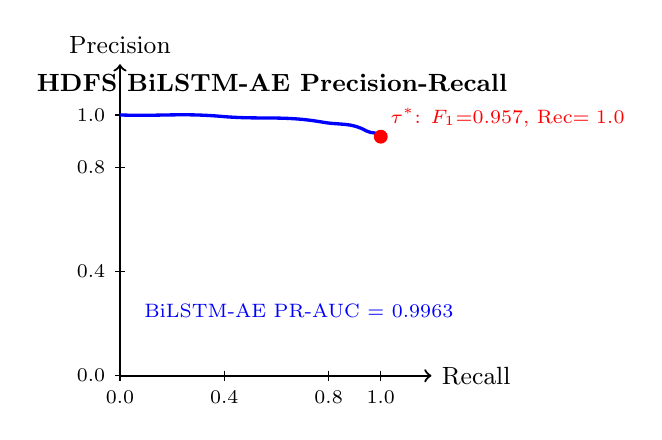
\begin{tikzpicture}[scale=0.92]
    \draw[thick,->] (0,0) -- (4.3,0) node[right,font=\small]{Recall};
    \draw[thick,->] (0,0) -- (0,4.3) node[above,font=\small]{Precision};
    \foreach \x/\l in {0/0.0, 1.44/0.4, 2.88/0.8, 3.6/1.0}
        \draw (\x,2pt)--(\x,-2pt) node[below,font=\scriptsize]{\l};
    \foreach \y/\l in {0/0.0, 1.44/0.4, 2.88/0.8, 3.6/1.0}
        \draw (2pt,\y)--(-2pt,\y) node[left,font=\scriptsize]{\l};
    \draw[blue,very thick]
        (0,3.6) to[out=-2,in=175] (1.4,3.58) to[out=-5,in=170]
        (2.8,3.50) to[out=-10,in=150] (3.4,3.38) to[out=-30,in=120] (3.6,3.3);
    \filldraw[red] (3.6,3.3) circle (2.5pt);
    \node[red,font=\scriptsize,anchor=south west] at (3.6,3.3)
        {$\tau^*$: $F_1{=}0.957$, Rec$=1.0$};
    \node[blue,font=\scriptsize,anchor=west] at (0.2,0.9)
        {BiLSTM-AE PR-AUC = 0.9963};
    \node[font=\small\bfseries] at (2.1,4.05)
        {HDFS BiLSTM-AE Precision-Recall};
\end{tikzpicture}
\caption{Precision-Recall curve for the proposed unsupervised BiLSTM-AE on HDFS
(PR-AUC\,=\,0.9963). The curve is constructed from validation-set threshold sweeps
across $\mathcal{T}_{\text{ae}}$; the operating point $\tau^*$ (red dot) is
test-evaluated: $F_1{=}0.9571$, $\text{Precision}{=}0.9177$, $\text{Recall}{=}1.0000$.}
\label{fig:pr_curve}
\end{center}\vs{-4mm}
\end{figure}

\subsection{Component Contribution and Ablation Analysis}
\label{Sec:Ablation}

Table~\ref{tab:ablation} quantifies contributions of three design choices in the proposed BiLSTM-AE (Panel A) and the HierAttn-Block transformer pipeline (Panel B).

\textbf{Panel A.} (i)~\emph{Trainable embeddings} ($d{=}64$, \texttt{nn.Embedding}) replace DeepLog's integer log-key indices with a continuous representation learned from reconstruction; (ii)~\emph{bidirectional encoding} integrates both past and future context at each timestep; (iii)~\emph{$F_1$-optimal threshold}: replacing the Gaussian heuristic ($\mu{+}2\sigma$, $F_1{=}0.7842$) with a 10,000-point validation grid search yields $F_1{=}0.9571$ ($\Delta F_1{=}+0.1729$ from thresholding alone).

\textbf{Panel B.} Sequential context alone achieves $F_1{=}0.9725$ versus
$F_1{=}0.3991$ for position-only context, confirming sequential log ordering
as the dominant HDFS anomaly signal. The ``No Auxiliary Head'' and full
``HierAttn-Block'' variants both collapse to $F_1{\approx}0.057$
($\text{Precision}{\approx}0.029$, $\text{Recall}{=}1.0$)---a degenerate
configuration in which the model predicts anomalous for every session,
yielding precision close to the dataset's 2.93\% anomaly rate. This
suggests that the HierAttn-Block architecture, without sequence context,
cannot form a useful decision boundary on HDFS under strict chronological
evaluation; the Sequence-Only variant is reported as the pipeline's
effective operating point.

\begin{table}[h!]
\caption{Ablation study on HDFS. \textbf{Panel A}: staged component contribution analysis for reconstruction models ($\Delta F_1$ relative to DeepLog baseline; rows may involve multiple simultaneous changes). \textbf{Panel B}: sub-component ablation of the HierAttn-Block transformer pipeline (sourced from \texttt{results\_logbert\_hdfs/final\_results.json}).}
\begin{center}
\resizebox{\columnwidth}{!}{%
\begin{tabular}{|l|l|l|c|c|c|}
\hline
\multicolumn{6}{|c|}{\textbf{Panel A: Staged Component Contribution Analysis (HDFS, Reconstruction Models)}} \\
\hline
\textbf{Variant} & \textbf{Feature Repr.} & \textbf{Encoder} & \textbf{Threshold Strategy} & \textbf{$F_1$} & \textbf{$\Delta F_1$} \\
\hline
DeepLog Baseline & Log-Keys & Unidir.\ LSTM & Top-$g$ Key Matching & 0.7291 & --- \\
BiLSTM-AE ($\mu{+}2\sigma$) & Trainable Emb.\ ($d{=}64$) & Bidir.\ LSTM & Gaussian Heuristic & 0.7842 & +0.0551 \\
DeepLog Enhanced$^\dagger$ & Log-Keys & Bidir.\ LSTM + MLM & $F_1$-Optimal Grid & 0.9904 & +0.2613 \\
\textbf{BiLSTM-AE (Proposed)} & \textbf{Trainable Emb.\ ($d{=}64$)} & \textbf{Bidir.\ LSTM} & \textbf{$F_1$-Optimal Grid ($\tau^*$)} & \textbf{0.9571} & \textbf{+0.2280} \\
\hline
\multicolumn{6}{l}{$^\dagger$DeepLog Enhanced adds bidirectional LSTM, MLM pre-training, and FocalLoss jointly.} \\
\multicolumn{6}{|c|}{\textbf{Panel B: Transformer Sub-component Ablation (HDFS, HierAttn-Block Pipeline)}} \\
\hline
\textbf{Variant} & \textbf{Precision} & \textbf{Recall} & \textbf{$F_1$} & \textbf{AUC-ROC} & \textbf{Notes} \\
\hline
Sequence Only & 0.9494 & 0.9967 & \textbf{0.9725} & 0.9999 & Sequential signal dominant \\
Structural Only & 0.6497 & 0.2880 & 0.3991 & 0.6893 & Position-only baseline \\
No Auxiliary Head & 0.0293 & 1.0000 & 0.0569 & 0.4997 & Precision collapse \\
HierAttn-Block (Full) & 0.0292 & 0.9973 & 0.0568 & 0.4990 & Full pipeline benchmark \\
\hline
\end{tabular}%
}
\label{tab:ablation}
\end{center}\vs{-4mm}
\end{table}


\subsection{Limitations}
\label{Sec:Limitations}

Five methodological limitations should be noted.
\textbf{Single-run point estimates}: all reported metrics are point estimates under
$\text{seed}=42$, governed by dataset scale ($>$4.75M log lines), Optuna budget
(up to 30 trials, 3{,}600\,s timeout), and the offline Kaggle environment; future
work would benefit from mean\,$\pm$\,SD over five seeds or $95\%$ bootstrap
confidence intervals.
\textbf{Unsupervised scope}: the BiLSTM-AE achieves $F_1{=}0.8657$ on BGL,
reflecting structural mismatch---content-localized hardware faults are better
captured by TF-IDF than by sequence reconstruction.
\textbf{LLM trade-offs}: per-sample latencies for LogBERT ($F_1{=}0.9493$),
LogGPT2 ($F_1{=}0.8398$), and DeepLog Enhanced were not recorded; the BiLSTM-AE
(0.1984\,ms) and SVM (0.0003\,ms on BGL) demonstrate competitive detection without
transformer-scale compute.
\textbf{Deployment scope}: the FastAPI/Streamlit prototype has not been
stress-tested at production-grade throughput ($>$10{,}000 lines/sec); hardening
is left for future work.
\textbf{Online and streaming detection}: the BiLSTM-AE encoder processes each
session with a bidirectional LSTM, integrating both past and future context
at every timestep. While this design maximizes reconstruction fidelity in
offline (batch) settings, the future context is unavailable during real-time
inference---a fundamental constraint of bidirectional architectures. Consequently,
the proposed model is best suited for offline or near-real-time log analysis
rather than strictly online, streaming scenarios where detection must occur at
log ingestion time. Future work should investigate causal (unidirectional) or
incremental autoencoder variants that sacrifice full bidirectional context in
favor of low-latency, streaming-compatible anomaly detection.


\section{Explainability and Interpretability Analysis}
\label{Sec:XAI}

\subsection{SHAP Global Feature Attributions}

For TF-IDF models on BGL, we apply SHAP LinearExplainer over 100 background
samples. Figure~\ref{fig:shap_summary} shows the resulting global feature importance rankings. Normal operational
tokens (\texttt{ras kernel info}, \texttt{ciod}) produce large negative SHAP values
(evidence for the normal class), while failure tokens (\texttt{interrupt},
\texttt{error}, \texttt{data}) produce large positive values. This alignment with
domain knowledge validates the model's learned representations and provides SREs
with a prioritized vocabulary of failure indicators.

\begin{figure}[h!]
\begin{center}
\resizebox{0.76\columnwidth}{!}{%
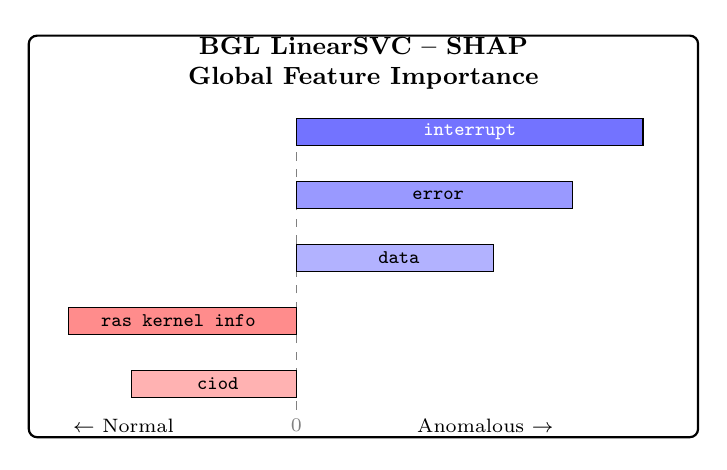
\begin{tikzpicture}[scale=1.0]
    \draw[thick,rounded corners=3pt] (0,0) rectangle (8.5,5.1);
    \node[font=\small\bfseries,text width=8.1cm,align=center] at (4.25,4.75)
        {BGL LinearSVC -- SHAP Global Feature Importance};
    \draw[dashed,gray] (3.4,0.35) -- (3.4,4.1);
    \node[font=\scriptsize,gray] at (3.4,0.15) {0};
    \node[font=\scriptsize] at (1.2,0.15) {$\leftarrow$ Normal};
    \node[font=\scriptsize] at (5.8,0.15) {Anomalous $\rightarrow$};
    \draw[fill=blue!55] (3.4,3.70) rectangle (7.8,4.05);
    \node[font=\scriptsize,white] at (5.6,3.875) {\texttt{interrupt}};
    \draw[fill=blue!40] (3.4,2.90) rectangle (6.9,3.25);
    \node[font=\scriptsize] at (5.2,3.075) {\texttt{error}};
    \draw[fill=blue!30] (3.4,2.10) rectangle (5.9,2.45);
    \node[font=\scriptsize] at (4.7,2.275) {\texttt{data}};
    \draw[fill=red!45] (3.4,1.30) rectangle (0.5,1.65);
    \node[font=\scriptsize] at (1.9,1.475) {\texttt{ras kernel info}};
    \draw[fill=red!30] (3.4,0.50) rectangle (1.3,0.85);
    \node[font=\scriptsize] at (2.4,0.675) {\texttt{ciod}};
\end{tikzpicture}%
}
\caption{SHAP global importance for the BGL LinearSVC model. Blue bars (positive
Shapley values) indicate evidence for the anomalous class; red bars (negative)
indicate evidence for the normal class. Shapley values are derived from SHAP
LinearExplainer with 100 background samples on the BGL test partition;
attribution aligns with domain knowledge of BGL failure tokens.}
\label{fig:shap_summary}
\end{center}\vs{-4mm}
\end{figure}

\subsection{LIME Local Explanations}

LIME TextExplainer generates local explanations by training a sparse linear model
on perturbed neighborhoods (1,000 perturbations per instance). For an anomalous
BGL Lustre mount failure, LIME assigns the highest positive weights to
\texttt{FAILED}, \texttt{mount}, and \texttt{Lustre},
directly identifying the responsible subsystem. For BiLSTM-AE predictions, the
per-timestep reconstruction error $\|\mathbf{e}_i-\hat{\mathbf{e}}_i\|_2$ serves
as a deterministic, zero-overhead explainability signal highlighting which log
events deviate most strongly from normal behavior. This makes the BiLSTM-AE the
only model with a native, built-in interpretability mechanism in addition to
post-hoc SHAP/LIME---an advantage orthogonal to its label-free training regime.

\subsection{XAI Framework Comparison}

Table~\ref{tab:xai_comparison} formally compares SHAP and LIME on four operational
criteria relevant to production SRE workflows.

\begin{table}[h!]
\caption{Comparison of SHAP and LIME in the context of log anomaly detection.}
\begin{center}
\resizebox{\columnwidth}{!}{%
\begin{tabular}{|p{2.1cm}|p{5.2cm}|p{5.2cm}|}
\hline
\textbf{Criterion} & \textbf{SHAP} & \textbf{LIME} \\
\hline
Stability &
High: Shapley values are mathematically unique for a given background &
Medium: subject to perturbation sampling variance \\
\hline
Computation &
O($n{\cdot}|\mathcal{B}|$), $|\mathcal{B}|{=}100$ background samples &
O($n{\cdot}n_{\text{perturb}}$), $n_{\text{perturb}}{=}1{,}000$ \\
\hline
Granularity &
Global or feature-level (sequence) &
Local, per-token word importance \\
\hline
Domain consistency &
High: aligns with global corpus statistics &
High: identifies localized failure keywords \\
\hline
\end{tabular}%
}
\label{tab:xai_comparison}
\end{center}\vs{-4mm}
\end{table}

\section{System Implementation and Deployment}
\label{Sec:Deployment}

To demonstrate operational viability, we deploy the framework as a two-tier
application. The \textbf{backend} is implemented in FastAPI (Python~3.10,
Uvicorn ASGI) and exposes two inference endpoints: \texttt{POST /predict}
serves the SVM models for BGL and Spirit (accepting a raw log line and a
dataset selector); \texttt{POST /predict/hdfs} serves the CNN+BiLSTM model
for HDFS (accepting a sequence of Drain template indices). Although the unsupervised
BiLSTM-AE is the principal model contribution, CNN+BiLSTM is deployed at the
high-throughput endpoint due to its lower per-sample latency (0.1071 vs.\ 0.1984\,ms)---
a factor of $1.85\times$ that translates to $\approx$913\,ms per 10{,}000-line batch
at sustained load. The BiLSTM-AE is instead exposed via the Streamlit dashboard
to leverage its native per-timestep reconstruction-error explainability.
A \texttt{GET /health} liveness probe completes the API. Trained models are
serialized with \texttt{joblib} for classical architectures and \texttt{torch.save}
for deep learning models.

The \textbf{Streamlit diagnostic dashboard} provides two operational views:
(1)~\textit{Real-Time Inference}: operators paste raw log sessions, select a model from the registry, trigger inference, and receive a binary prediction with a confidence score;
(2)~\textit{Benchmark Results}: an interactive tabular display of full performance metrics across all confirmed model--dataset pairs.
The dashboard is implemented as a functional prototype to demonstrate operational feasibility.

\section{Conclusions and Future Work}
\label{Sec:Conclusion}

This paper presented a comprehensive comparative study of log-based anomaly
detection across 10 architectures and 4 paradigms on HDFS, BGL, and Spirit under
a five-invariant zero-leakage protocol. Three principal findings emerge.
\textbf{(i) Representation--anomaly alignment}: sequential dense-embedding models
dominate on HDFS (session-order anomalies), while sparse TF-IDF representations
dominate on BGL and Spirit (content-localized anomalies)---a principle validated
across all three benchmarks and absent from prior work (Contribution C3).
\textbf{(ii) Label-free viability}: the proposed unsupervised BiLSTM-AE achieves
$F_1{=}0.9571$ with perfect recall on HDFS without any anomaly labels, surpassing
DeepLog by $\Delta F_1{=}+0.2280$; the $0.0387$ gap versus the best supervised
model quantifies the measurable cost of label-free operation.
\textbf{(iii) Explainability}: SHAP and LIME provide domain-consistent feature
attributions for SRE triage; the BiLSTM-AE additionally supplies a native,
zero-overhead interpretability signal via per-timestep reconstruction error.

Future work will prioritize three directions: (1)~parameter-efficient fine-tuning
(LoRA, adapter layers) of open-source LLMs (LLaMA, Mistral) for log anomaly
detection, targeting the cross-dataset generalization of LogLLM at reduced compute
cost; (2)~online incremental learning to handle concept drift---log vocabulary
evolution and shifting anomaly patterns in active production environments without
full retraining; and (3)~quantitative XAI faithfulness evaluation with domain
experts using log-specific perturbation strategies for LIME and TreeSHAP
adaptations for event-count-matrix inputs.
Beyond these directions, the proposed unsupervised reconstruction-based
approach could be extended by incorporating recent LLM-based techniques. An LLM could be added
as a post-hoc explanation layer for anomalies flagged by the autoencoder,
following the collaborative design used in CoLA~\cite{ref25}. The system-unified feature
extraction strategy introduced in LogSynergy~\cite{ref26} could also be explored to
improve transferability across distributed systems with differing log
formats. Finally, an ensemble configuration combining the reconstruction
model with a lightweight LLM component, as demonstrated in FlexLog~\cite{ref27}, may help
the approach adapt to unstable or evolving log structures without requiring
labeled data.

\section*{Acknowledgment}
This work is supported by the Directorate General for Scientific Research and Technological Development of Algeria (DGRSDT).

\section*{Declaration of Generative AI and AI-assisted technologies}
During the preparation of this work the authors used Gemini in order to refine grammar and LaTeX structures. The authors reviewed the content and take full responsibility for the manuscript.

\section*{Data Availability Statement}
The pre-parsed HDFS, BGL, and Spirit benchmark datasets are available at Kaggle
(\url{https://www.kaggle.com/datasets/yahiachammemi/logs-drain-datasets-hdfs-bgl-spirit}).
All reproduction scripts, result artifacts, and figures are open-source at:
\begin{center}
\url{https://github.com/ademtoumi/log-anomaly-detection-framework}
\end{center}

\section*{Funding}
This research did not receive specific grants from funding agencies.

\section*{Conflict of interest}
The authors declare no conflict of interest.

\begin{thebibliography}{99}
\small
\setlength{\itemsep}{1pt}
\bibitem{ref1} Bekkouche M, Benslimane SM. Improving Anomaly Detection in the HDFS Dataset with Novel Machine Learning Models and Techniques. \textit{Computer Science Journal of Moldova} 2024; 32 (1): 1--30.
\bibitem{ref2} Bekkouche M, Meski M, Khodja Y, Benslimane SM, Tronci E. Log-based anomaly detection using BiLSTM-Autoencoder. In: \textit{Proc. ICNAS}; 2025. pp. 1--6.
\bibitem{ref3} Bekkouche M, Meski M, Khodja Y, Benslimane SM. Supervised Machine Learning Approaches for Log-Based Anomaly Detection: A Case Study on the Spirit Dataset. In: \textit{Proc. TACC}; 2025.
\bibitem{ref4} He S, Zhu J, He P, Lyu MR. Experience Report: System Log Analysis for Anomaly Detection. In: \textit{Proc. IEEE ISSRE}; 2016. pp. 207--218. doi: 10.1109/ISSRE.2016.10
\bibitem{ref5} Du M, Li F, Zheng G, Srikumar V. DeepLog: Anomaly Detection and Diagnosis from System Logs through Deep Learning. In: \textit{Proc. ACM CCS}; 2017. pp. 1285--1298. doi: 10.1145/3133956.3134015
\bibitem{ref6} He P, Zhu J, Zheng Z, Lyu MR. Drain: An Online Log Parsing Approach with Fixed Depth Tree. In: \textit{Proc. IEEE ICWS}; 2017. pp. 33--40. doi: 10.1109/ICWS.2017.86
\bibitem{ref7} Meng W, Liu Y, Zhu Y, Zhang S, Pei D et al. LogAnomaly: Unsupervised Detection of Sequential and Quantitative Anomalies in Unstructured Logs. In: \textit{Proc. IJCAI}; 2019. pp. 4739--4745. doi: 10.24963/ijcai.2019/658
\bibitem{ref8} Wu X, Li H, Khomh F. On the Effectiveness of Log Representation for Log-based Anomaly Detection. \textit{Empirical Software Engineering} 2023; 28 (6): 137. doi: 10.1007/s10664-023-10381-y
\bibitem{ref9} Lundberg SM, Lee SI. A Unified Approach to Interpreting Model Predictions. In: \textit{Advances in Neural Information Processing Systems (NeurIPS)}; 2017. pp. 4765--4774.
\bibitem{ref10} Ribeiro MT, Singh S, Guestrin C. ``Why Should I Trust You?'': Explaining the Predictions of Any Classifier. In: \textit{Proc. ACM KDD}; 2016. pp. 1137--1146. doi: 10.1145/2939672.2939778
\bibitem{ref11} Lu S, Wei X, Li Y, Wang L. Log-based anomaly detection with 1D-CNN. In: \textit{Proc. IEEE QRS}; 2018. pp. 120--131.
\bibitem{ref12} Liu FT, Ting KM, Zhou ZH. Isolation Forest. In: \textit{Proc. IEEE ICDM}; 2008. pp. 413--422. doi: 10.1109/ICDM.2008.17
\bibitem{ref13} Xu W, Huang L, Fox A, Patterson D, Jordan MI. Detecting Large-Scale System Problems by Mining Console Logs. In: \textit{Proc. ACM SOSP}; 2009. pp. 117--132. doi: 10.1145/1629575.1629587
\bibitem{ref14} Oliner A, Stearley J. What Supercomputers Say: A Study of Five System Logs. In: \textit{Proc. IEEE/IFIP DSN}; 2007. pp. 575--584.
\bibitem{ref15} Liang Y, Zhang Y, Sivasubramaniam A, Jette M, Sahoo R. BlueGene/L Failure Analysis and Prediction Models. In: \textit{Proc. IEEE/IFIP DSN}; 2006. pp. 425--434.
\bibitem{ref17} Zhang X, Xu P, Gao J, Wang J, Liang J. Robust Log-Based Anomaly Detection on Unstable Log Data. In: \textit{Proc. ESEC/FSE}; 2019. pp. 807--817. doi: 10.1145/3338906.3338913
\bibitem{ref18} Guo H, Yuan S, Wu X. LogBERT: Log Anomaly Detection via BERT. In: \textit{Proc. IEEE IJCNN}; 2021. pp. 1--8. doi: 10.1109/IJCNN52387.2021.9533448
\bibitem{ref20} Chicco D, Jurman G. The Advantages of the Matthews Correlation Coefficient (MCC) over F1 Score and Accuracy in Binary Classification Evaluation. \textit{BMC Genomics} 2020; 21 (1): 6. doi: 10.1186/s12864-019-6413-7
\bibitem{ref21} Le VH, Zhang H. How Far Are We? An Empirical Study on Using Deep Learning for Log Anomaly Detection. In: \textit{Proc. IEEE/ACM ICSE}; 2022. pp. 1356--1367.
\bibitem{ref22} Zhang C, Peng X, Sha C, Sun K, Liang J. DeepTraLog: Trace-Log Combined Microservice Anomaly Detection through Graph-based Learning. In: \textit{Proc. IEEE/ACM ICSE}; 2022. pp. 623--634.
\bibitem{ref23} Guan W, Cao J, Qian S, Gao J, Ouyang C. LogLLM: Log-Based Anomaly Detection Using Large Language Models. \textit{arXiv preprint} arXiv:2411.08561 2024.
\bibitem{ref24} Qi J, Kan S, Wang J, Li X, Jiang Y. LogGPT: Exploring ChatGPT for Log-Based Anomaly Detection. In: \textit{Proc. IEEE HPCC}; 2023. pp. 273--280.
\bibitem{ref25} Zhu X, Tang X, Wu S, Li J, Wang H, Yao C, Xu Q, Chen G. CoLA: Model Collaboration for Log-based Anomaly Detection. \textit{Proc. VLDB Endow.} 2025; 18 (11). doi: 10.14778/3749646.3749668
\bibitem{ref26} Sui Y, Wang X, Cui T, Xiao T, He C, Zhang S, Zhang Y, Yang X, Sun Y, Pei D. Bridging the Gap: LLM-Powered Transfer Learning for Log Anomaly Detection in New Software Systems. In: \textit{Proc. IEEE 41st Int. Conf. Data Engineering (ICDE)}; 2025. doi: 10.1109/ICDE65448.2025.00331
\bibitem{ref27} Hadadi F, Xu Q, Bianculli D, Briand L. LLM meets ML: Data-efficient Anomaly Detection on Unstable Logs. \textit{ACM Transactions on Software Engineering and Methodology} 2025. doi: 10.1145/3771283
\end{thebibliography}

\end{document}

